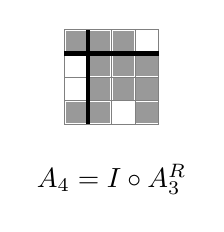
\begin{tikzpicture}
\draw[step=0.3cm,gray,thin] (0,0) grid (1.2,1.2);
\fill[black!40!white] (0.015,1.185) rectangle (0.285,0.9149999999999999);
\fill[black!40!white] (0.315,1.185) rectangle (0.585,0.9149999999999999);
\fill[black!40!white] (0.6149999999999999,1.185) rectangle (0.885,0.9149999999999999);
\fill[black!40!white] (0.315,0.885) rectangle (0.585,0.6149999999999999);
\fill[black!40!white] (0.6149999999999999,0.885) rectangle (0.885,0.6149999999999999);
\fill[black!40!white] (0.9149999999999999,0.885) rectangle (1.185,0.6149999999999999);
\fill[black!40!white] (0.315,0.585) rectangle (0.585,0.315);
\fill[black!40!white] (0.6149999999999999,0.585) rectangle (0.885,0.315);
\fill[black!40!white] (0.9149999999999999,0.585) rectangle (1.185,0.315);
\fill[black!40!white] (0.015,0.285) rectangle (0.285,0.015000000000000013);
\fill[black!40!white] (0.315,0.285) rectangle (0.585,0.015000000000000013);
\fill[black!40!white] (0.9149999999999999,0.285) rectangle (1.185,0.015000000000000013);
\draw[ultra thick] (0.3,0.0) -- (0.3,1.2);
\draw[ultra thick] (0.0,0.8999999999999999) -- (1.2,0.8999999999999999);
\node[] at (0.6,-0.7) {  $A_{4}=I \circ A_3^R$};\end{tikzpicture}